\documentclass[9pt,a4paper]{article}

\usepackage[margin=1.5cm]{geometry}
\usepackage{enumitem}
\usepackage{array}
\usepackage{tabularx}
\usepackage{tikz}
\usepackage{titlesec}
\usetikzlibrary{arrows.meta,positioning}

\setlength{\parindent}{0pt}
\setlength{\parskip}{0.2em}
\setlist[itemize]{leftmargin=1.4em,itemsep=0pt,topsep=1pt}
\setlist[enumerate]{leftmargin=1.5em,itemsep=0pt,topsep=1pt}
\renewcommand{\arraystretch}{1.0}
\newcolumntype{Y}{>{\raggedright\arraybackslash}X}
\titlespacing*{\section}{0pt}{0.7em}{0.25em}
\titlespacing*{\subsection}{0pt}{0.45em}{0.15em}

\begin{document}

\begin{center}
  {\large\textbf{AGENTRIX 2026 National AI Hackathon}}\\[0.25em]
  {\large\textbf{TEAM PROPOSAL DOCUMENT}}\\[0.5em]
\end{center}

\begin{tabularx}{\textwidth}{@{}lY@{}}
\textbf{Product Name:} & Cura \\
\textbf{Team Name:} & Lua \\
\textbf{Team ID:} & Lua-JainUniversity \\
\textbf{Team Members:} & Aryan Soni, Akshat Gupta, Aadvik Raj, Aman \\
\textbf{Problem Statement:} & Problem Statement 6: CareCompanion - AI Mental Health Support for Remote Communities \\
\textbf{Submission Time:} & 10:50 AM \quad (Submission deadline: 11:00 AM) \\
\end{tabularx}

\section*{1. Problem Understanding}

\subsection*{1.1 Problem Statement}

Mental health crises are accelerating globally, but psychological services are
severely constrained. One in eight people globally are affected by mental
health disorders, while low-income countries have only one psychologist per
100,000 people. Stigma prevents many people from seeking help, and crisis
intervention services are often unavailable in rural areas. Suicide rates are
also climbing, especially among youth and farmers. Rural communities face
additional barriers: qualified therapists may be far away, therapy can be
expensive, and unreliable internet makes regular online care difficult. People
may also avoid local clinics because they fear being recognised. Cura aims to
provide an accessible first point of mental health support in a private space,
while directing people to human professionals when serious risk is detected.

\subsection*{1.2 Existing Challenges}

\begin{itemize}
  \item \textbf{Limited access:} Rural areas often do not have enough
        qualified therapists or crisis services.
  \item \textbf{Stigma:} People may avoid therapy because they do not want
        others to know they are seeking help.
  \item \textbf{Cost:} Regular therapy is unaffordable for many individuals and
        families.
  \item \textbf{Weak connection:} Text-only applications do not provide the
        eye contact, facial movement and listening cues of a human conversation.
\end{itemize}

\subsection*{1.3 Target Users}

\textbf{Primary Users:} People in remote and rural communities, especially
youth, farmers and individuals who cannot easily access a therapist.\\
\textbf{Secondary Users:} Community health workers, counsellors and families
who need a way to support people between professional appointments.

\section*{2. Proposed Solution}

\subsection*{2.1 Solution Overview}

Our solution, \textbf{Cura}, is a browser-based AI mental health companion
centred around an interactive 3D avatar. A user can speak about their feelings
and receive a spoken response from the avatar. The model uses live lip movement,
eye contact, facial expressions and listening gestures to make the conversation
feel more personal than a normal chatbot. This gives users a private way to
access basic support from their own space, without travelling to a clinic or
paying for every conversation.

The user audio is transcribed and sent to a language model through OpenRouter.
The response is streamed sentence by sentence to reduce waiting time. Google
Cloud Text-to-Speech generates the voice and word timings. TalkingHead uses
those timings to animate the avatar's mouth in real time. Cura can guide
breathing and grounding exercises, ask wellbeing questions, and identify
possible crisis language. When serious risk is detected, it presents crisis
resources and recommends contact with a real counsellor. Cura supports human
care rather than replacing professional therapy.

\subsection*{2.2 Key Features}

\begin{tabularx}{\textwidth}{@{}p{3.4cm}Y@{}}
\textbf{Feature} & \textbf{Description} \\
\hline
3D speaking avatar & Real-time lip-sync, eye contact, facial movement and
listening gestures using a GLB model. \\
Private access & Users can access support from their own personal space through
a browser. \\
AI conversation & Supportive responses, sentence streaming and mood-aware
conversation. \\
Guided activities & Breathing, grounding and simple wellbeing check-ins. \\
Safety response & Risk detection, crisis resources and recommendation for human
support. \\
\end{tabularx}

\section*{3. AI / Agentic Approach}

\subsection*{3.1 AI Components}

\begin{itemize}
  \item \textbf{Large Language Model:} OpenRouter provides access to a
        conversational model with streaming output.
  \item \textbf{AI Agents:} A conversation agent generates responses; a safety
        agent classifies risk; an avatar controller selects mood and gestures.
  \item \textbf{RAG:} A small curated resource list can provide local helpline
        and emergency information.
  \item \textbf{Machine Learning:} No custom model is required for the MVP.
  \item \textbf{Computer Vision:} Not used in the MVP.
  \item \textbf{NLP:} Speech recognition, intent understanding, risk detection
        and response generation.
  \item \textbf{Other:} Google Cloud TTS provides audio and word timings for
        lip-sync.
\end{itemize}

\subsection*{3.2 Agent Workflow}

\begin{center}
\texttt{User Speech -> Transcription -> Intent and Risk Analysis -> Response Agent}
\end{center}
\begin{center}
\texttt{-> Safety Check -> TTS and Visemes -> 3D Avatar Response}
\end{center}

The microphone captures a user turn and speech recognition converts it to text.
The safety component checks for crisis signals while the conversation agent
prepares a response. The response is passed to Google TTS, which returns audio
and word timings. TalkingHead converts the timings into visemes and animates the
avatar. If the safety result indicates serious risk, the normal response is
replaced or supplemented with crisis guidance and human-support options.

\section*{4. System Architecture}

\begin{center}
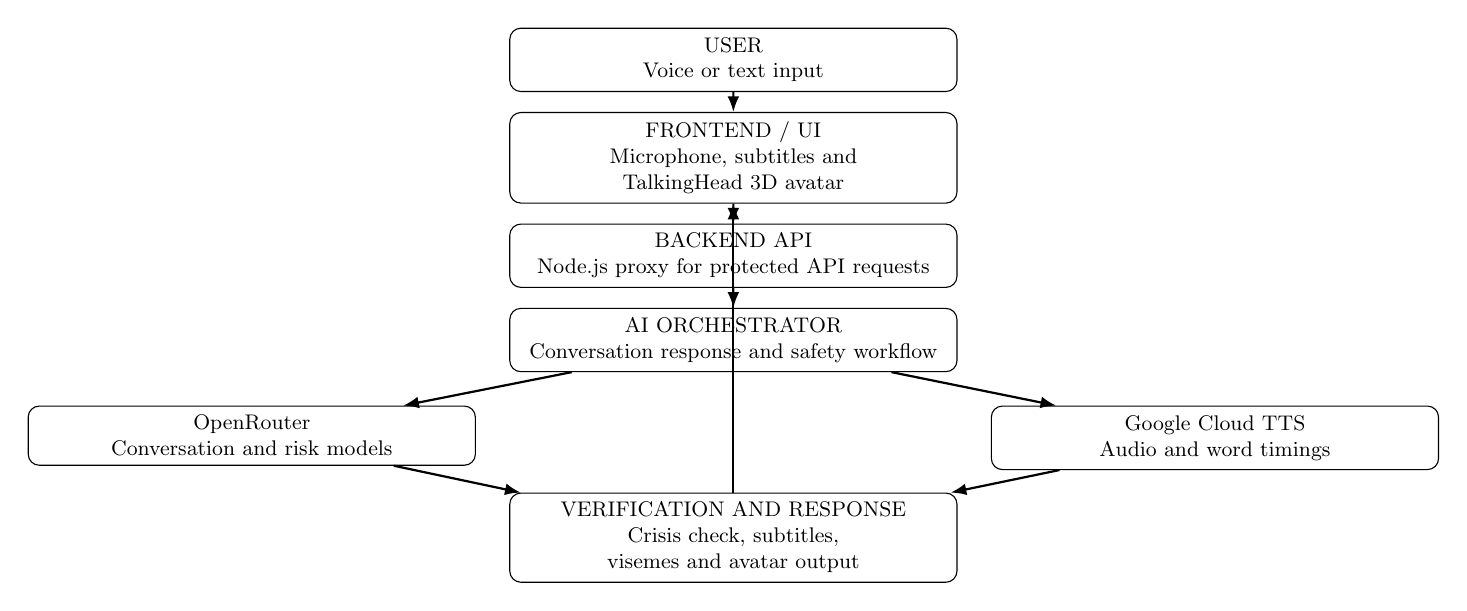
\begin{tikzpicture}[
  scale=0.85, transform shape,
  box/.style={draw, rounded corners, align=center, text width=6.4cm,
              inner sep=4pt, font=\small},
  flow/.style={-{Latex[length=2mm]}, thick}
]
  \node[box] (user) {USER\\Voice or text input};
  \node[box, below=3mm of user] (front) {FRONTEND / UI\\Microphone, subtitles and TalkingHead 3D avatar};
  \node[box, below=3mm of front] (back) {BACKEND API\\Node.js proxy for protected API requests};
  \node[box, below=3mm of back] (orch) {AI ORCHESTRATOR\\Conversation response and safety workflow};
  \node[box, below left=5mm and 5mm of orch] (llm) {OpenRouter\\Conversation and risk models};
  \node[box, below right=5mm and 5mm of orch] (tts) {Google Cloud TTS\\Audio and word timings};
  \node[box, below=18mm of orch] (result) {VERIFICATION AND RESPONSE\\Crisis check, subtitles, visemes and avatar output};

  \draw[flow] (user) -- (front);
  \draw[flow] (front) -- (back);
  \draw[flow] (back) -- (orch);
  \draw[flow] (orch) -- (llm);
  \draw[flow] (orch) -- (tts);
  \draw[flow] (llm) -- (result);
  \draw[flow] (tts) -- (result);
  \draw[flow] (result) -- (front);
\end{tikzpicture}
\end{center}

\section*{5. Innovation}

Cura focuses on the part of a mental health conversation that text-based
applications cannot provide: a sense of presence. The 3D avatar uses live
lip-sync, eye contact, facial movement and listening gestures to build a more
natural connection with the user. This is particularly useful for people who
may not feel comfortable visiting a local clinic because of stigma. Cura also
combines the avatar with a private browser experience, which allows support to
be accessed from the user's own space. AI is needed to understand free-form
conversation, respond appropriately and detect risk signals. The system is not
intended to diagnose or replace a therapist. Its unique role is to provide
support, basic guided activities and a path to human help between professional
visits.

\section*{6. Technology Stack}

\begin{tabularx}{\textwidth}{@{}p{3.2cm}Y@{}}
\textbf{Layer} & \textbf{Technology} \\
\hline
Frontend & Next.js, JavaScript, three.js, WebGL and TalkingHead \\
Backend & Node.js with a small API proxy \\
Database & IndexedDB for local browser storage; no remote database in the MVP \\
AI / LLM & OpenRouter conversational and safety models \\
AI Framework & Direct API integration; no framework required for the MVP \\
Vector Database & Not required for the MVP \\
APIs / Tools & Google Cloud TTS, browser speech recognition, TalkingHead and
Ready Player Me GLB avatar \\
Deployment & Static frontend on Vercel with backend API routes \\
\end{tabularx}

\section*{7. MVP Scope}

\textbf{Must Have}
\begin{itemize}
  \item [ ] 3D avatar with working lip-sync
  \item [ ] Voice input and speech recognition
  \item [ ] OpenRouter conversation integration
  \item [ ] Google TTS with word timings
  \item [ ] Crisis-risk response and resource display
  \item [ ] Working frontend, backend proxy and end-to-end deployment
\end{itemize}

\textbf{Nice to Have}
\begin{itemize}
  \item [ ] Guided breathing and grounding exercises
  \item [ ] Conversational PHQ-9 and GAD-7 check-ins
  \item [ ] Mood history and personalisation
  \item [ ] Local-language support and human counsellor handoff
\end{itemize}

\section*{8. Expected User Flow}

\begin{enumerate}
  \item User opens Cura and clicks ``Start Session''.
  \item User speaks about a concern or selects a guided activity.
  \item Speech is transcribed and analysed for intent and safety risk.
  \item The response agent generates a short supportive response.
  \item Google TTS produces speech and word timings.
  \item The 3D avatar speaks with synchronised lip movement and subtitles.
  \item Crisis resources are shown when the safety check requires them.
\end{enumerate}

\textbf{Example User Scenario}\\
\textbf{User:} ``I feel overwhelmed and cannot sleep.''\\
\textbf{System:} Transcribes the statement, checks risk, and prepares a
supportive response with an optional breathing exercise.\\
\textbf{Final Output:} The avatar speaks the response with live lip-sync and
shows subtitles. If a crisis signal is detected, relevant human-support
resources are displayed.

\section*{9. Expected Impact}

\begin{tabularx}{\textwidth}{@{}p{3.2cm}Y@{}}
\textbf{Benefit} & \textbf{Expected value} \\
\hline
Access & Provides an available first point of support for people far from
therapists. \\
Privacy & Allows users to seek support from their own personal space. \\
Cost reduction & Offers basic support between paid professional sessions. \\
User experience & Uses a speaking, responsive avatar rather than only text. \\
Scalability & A browser-based service can support many users with the same core
system. \\
\end{tabularx}

Cura can help reduce the gap between a person's need for support and the next
available human appointment. It is most valuable as a bridge to professional
care, with crisis escalation built into the experience.

\section*{10. Implementation Plan}

\begin{tabularx}{\textwidth}{@{}p{3cm}Yp{3.2cm}@{}}
\textbf{Phase} & \textbf{Activity} & \textbf{Responsible Member(s)} \\
\hline
Phase 1 & Requirements and architecture & Akshat Gupta \\
Phase 2 & Backend and API setup & Aryan Soni \\
Phase 3 & Conversation and safety workflow & Aadvik Raj, Aman \\
Phase 4 & 3D avatar and frontend & Aryan Soni \\
Phase 5 & Integration and lip-sync testing & Aadvik Raj, Aman \\
Phase 6 & Testing and deployment & Aryan Soni \\
Phase 7 & Demo and documentation & Akshat Gupta \\
\end{tabularx}

\section*{11. Risks and Mitigation}

\begin{tabularx}{\textwidth}{@{}p{3.4cm}p{2cm}Y@{}}
\textbf{Risk} & \textbf{Impact} & \textbf{Mitigation} \\
\hline
API or network failure & High & Use provider fallback and keep a local demo backup. \\
Unsafe AI response & High & Use a separate risk check, restricted prompts and fixed crisis responses. \\
Lip-sync integration issue & Medium & Validate the avatar and TTS pipeline before adding other features. \\
Time constraints & High & Keep the MVP focused on avatar, voice, response and safety. \\
Deployment failure & Medium & Deploy a basic version early and keep a local demo backup. \\
\end{tabularx}

\section*{12. Success Criteria}

The solution will be considered successful if:
\begin{itemize}
  \item [ ] The avatar speaks with visible lip-sync.
  \item [ ] A user can complete a voice conversation end-to-end.
  \item [ ] AI produces useful and supportive responses.
  \item [ ] Risk detection displays appropriate crisis guidance.
  \item [ ] The application is functional and deployed.
  \item [ ] The complete workflow can be demonstrated successfully.
\end{itemize}

\section*{13. Demo Plan}

\textbf{Input:} A user says, ``I am stressed and need help calming down.''\\
\textbf{AI Processing:} Speech recognition creates a transcript. OpenRouter
generates a response and checks risk. Google TTS returns the voice and word
timings. TalkingHead animates the avatar.\\
\textbf{Output:} Cura responds through the 3D avatar, displays subtitles and
offers a short breathing exercise.

\begin{center}
\texttt{User Input -> AI Understanding -> Safety Check -> Response -> TTS -> 3D Avatar Output}
\end{center}

\section*{14. Team Details}

\begin{tabularx}{\textwidth}{@{}p{4cm}p{3.2cm}Y@{}}
\textbf{Name} & \textbf{Role} & \textbf{Responsibilities} \\
\hline
Aryan Soni & Team Lead & Coordination and integration \\
Aryan Soni & AI / ML & OpenRouter, prompts and safety workflow \\
Aryan Soni & Backend & API proxy and deployment \\
Akshat Gupta & Frontend & 3D avatar and user interface \\
Aman, Aadvik Raj, Akshat Gupta, Aryan Soni & UI / UX / QA & User flow, testing and presentation \\
\end{tabularx}

\enlargethispage{2cm}
\section*{15. Final Proposal Summary}

Our solution, Cura, addresses the lack of accessible mental health support in
remote communities. It uses OpenRouter for conversational AI, Google Cloud
Text-to-Speech for speech with word timings, and TalkingHead for a 3D avatar
with live lip-sync. Users can speak privately from their own space and receive
supportive responses, guided activities and crisis resources. Unlike a normal
chatbot, the avatar uses eye contact, facial movement and listening gestures to
create a stronger sense of connection. The hackathon MVP will demonstrate a
complete voice conversation from user speech to a spoken, animated response.

\subsection*{Submission Checklist}

\begin{itemize}
  \item [ ] Team and member details completed
  \item [ ] Problem understanding and solution included
  \item [ ] AI approach and architecture included
  \item [ ] Innovation and technology stack included
  \item [ ] MVP scope, user flow and impact included
  \item [ ] Implementation plan, risks and success criteria included
\end{itemize}

\end{document}
